\subsection{Mean squared error (MSE)}
Der naive Ansatz zwei Bilder auf visuelle Ähnlichkeit zu bewerten, ist es
iterativ alle Pixelintensitäten miteinander zu vergleichen. Als Werkzeug zum
Vergleich dient hierbei die \textit{mittlere quadratische Abweichung}\footnote{https://www.spektrum.de/lexikon/mathematik/mittlere-quadratische-abweichung/7033 [09.12.2022]}
(Mean squared error) \parencite{mse-overview}. Je niedriger die Abweichung
zwischen den Bildern, desto mehr stimmen sie überein. Obwohl dieses Verfahren 
verhältnismäßig leicht zu implementieren ist, ist es nur für Fälle geeignet,
bei denen sowohl das Referenz- als auch das Testbild fast identisch sind.
Bereits  kleinste Helligkeitsänderungen, bei gleichbleibendem Inhalt, ergeben
nach Berechnung, des \textit{euklidischen Abstands}\footnote{https://www.spektrum.de/lexikon/mathematik/euklidischer-abstand/4584 [09.12.2022]},
eine hohe mittlere quadratische Abweichung (siehe Abbildung
\ref{fig:mse-naive}). \parencite{mse-naive-approach}

\begin{figure}[H]
    \centering
    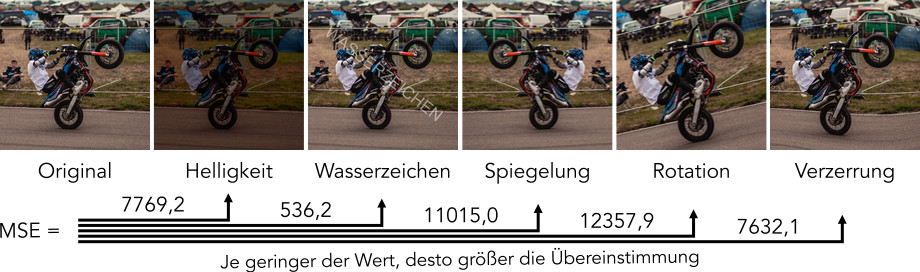
\includegraphics[width=\textwidth]{mse-naive-approach}
    \caption{MSE: Anwendung an verschiedenen Testbildern}
    \label{fig:mse-naive}
    \bildquelle{Eigene Darstellung}
\end{figure}